\let\negmedspace\undefined
\let\negthickspace\undefined
\documentclass[journal]{IEEEtran}
\usepackage[a5paper, margin=10mm, onecolumn]{geometry}
%\usepackage{lmodern} % Ensure lmodern is loaded for pdflatex
\usepackage{tfrupee} % Include tfrupee package

\setlength{\headheight}{1cm} % Set the height of the header box
\setlength{\headsep}{0mm}     % Set the distance between the header box and the top of the text

\usepackage{gvv-book}
\usepackage{gvv}
\usepackage{cite}
\usepackage{amsmath,amssymb,amsfonts,amsthm}
\usepackage{algorithmic}
\usepackage{graphicx}
\usepackage{textcomp}
\usepackage{xcolor}
\usepackage{txfonts}
\usepackage{listings}
\usepackage{enumitem}
\usepackage{mathtools}
\usepackage{gensymb}
\usepackage{comment}
\usepackage[breaklinks=true]{hyperref}
\usepackage{tkz-euclide} 
\usepackage{listings}
% \usepackage{gvv}                                        
\def\inputGnumericTable{}                                 
\usepackage[latin1]{inputenc}                                
\usepackage{color}                                            
\usepackage{array}                                            
\usepackage{longtable}                                       
\usepackage{calc}                                             
\usepackage{multirow}                                         
\usepackage{hhline}                                           
\usepackage{ifthen}                                           
\usepackage{lscape}
\begin{document}

\bibliographystyle{IEEEtran}
\vspace{3cm}

\title{3-3.4-1}
\author{EE24BTECH11010 - Balaji}
% \maketitle
% \newpage
% \bigskip
{\let\newpage\relax\maketitle}

\renewcommand{\thefigure}{\theenumi}
\renewcommand{\thetable}{\theenumi}
\setlength{\intextsep}{10pt} % Space between text and floats

\numberwithin{figure}{enumi}
\renewcommand{\thetable}{\theenumi}

\textbf{Question :} \\
Draw a quadrilateral in the Cartesian plane, whose vertices are \myvec{-4 \\  5}, \myvec{0\\ 7}, \myvec{5 \\ -5}
and \myvec{-4\\ -2} \\
\textbf{Answer :}\\
\begin{table}[h!]
      \centering
      \begin{tabular}[12pt]{ |c| c| c|c|c|c|}
    \hline
    $X$ & 1 & 2 & 3 & 4 & 5 \\
    \hline
    $P(X)$ & $K$ & 2$K$ & 2$K$ & 3$K$ & $K$ \\
    \hline 
    \end{tabular} 

      \caption{}
\end{table}

Length of the side $\vec{AB}$, $d_1$ is
\begin{align}
	\brak{\vec{A} - \vec{B}} = \myvec{-4\\5} - \myvec{0\\7} &= \myvec{-4\\-2}\\
	\brak{\vec{A-B}}^\top\brak{\vec{A-B}}&=20\\
    d_1=||\vec{A}-\vec{B}||&=\sqrt{20}
\end{align}
Length of the side $\vec{BC}$, $d_2$ is
\begin{align}
	\brak{\vec{B} - \vec{C}} = \myvec{0\\7} - \myvec{5\\-5} &= \myvec{-5\\12}\\
	\brak{\vec{B-C}}^\top\brak{\vec{B-C}}&=169\\
    d_2=||\vec{A}-\vec{O}||&=13
\end{align}
Length of the side $\vec{CD}$, $d_3$ is
\begin{align}
	\brak{\vec{C} - \vec{D}} = \myvec{5\\-5} - \myvec{-4\\-2} &= \myvec{9\\-3}\\
	\brak{\vec{C-D}}^\top\brak{\vec{C-D}}&=90\\
    d_3=||\vec{O}-\vec{B}||&=\sqrt{90}
\end{align}
Length of the side $\vec{DA}$, $d_4$ is
\begin{align}
	\brak{\vec{D} - \vec{A}} = \myvec{-4\\-2} - \myvec{-4\\5} &= \myvec{0\\-7}\\
	\brak{\vec{D-A}}^\top\brak{\vec{D-A}}&=49\\
    d_4=||\vec{O}-\vec{B}||&=7
\end{align}
Perimeter of the Quadrilateral is 
\begin{align}
    d_1+d_2+d_3+d_4&=\sqrt{20}+\sqrt{90}+20
\end{align}
The Quadrilateral formed by the points:
\begin{figure}[h!]
   \centering
   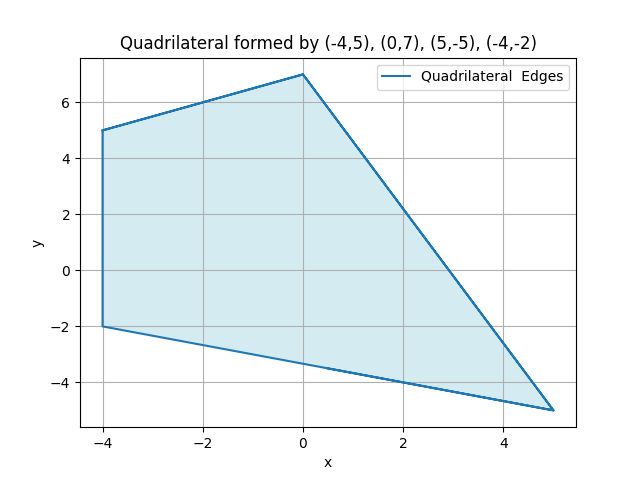
\includegraphics[width=0.7\linewidth]{figs/fig.png}
   \caption{Plot of the Quadrilateral}
   \label{stemplot}
\end{figure}  
\end{document}

